\section{Simulations}
\label{sec:simulations}
The following simulations of the dual-arm non-resonant antenna design are done in CST Microwave Studio using its time-domain solver, FIT (Finite Integral Technique). All matching components used are ideal and the simulations are carried out on a bare board, thus the traces from the tunable MEMS capacitor and SMA connectors are not included in the simulation. 
The antennas, in simplified simulations, are designed to resonate higher than desired as practice has shown detuning when moved to the PCB with MEMS tuners.
The simulations include $S$-parameters, correlation, efficiency in free-space, talk-mode, data-mode, and two-hand-mode. In addition, the peak specific absorption rate (SAR) values of the antenna structures next to a SAM (Specific Antropomorphic Mannequin) head phantom is simulated. The following plots are when sweeping the tuner from around \SI{0.6}{pF} to \SI{6}{pF} (top antenna) and from around \SI{1.2}{pF} to \SI{12}{pF} (side antenna).


%Free space S11 + S22 + Isolation i text
The simulated $S$-parameters are shown in Fig.~\ref{fig:sim_sparams}. Both antennas cover the low band at \SI{6}{dB} return loss. The high band is, however, not entirely covered. The top antenna covers from \SIrange{1760}{2550}{MHz} and the side antenna from \SIrange{1710}{2550}{MHz}. The isolation is a minimum of \SI{6}{dB} in the low band and generally higher for the high band with an isolation above \SI{13}{dB}. 
\begin{figure}[tb]
    \centering
    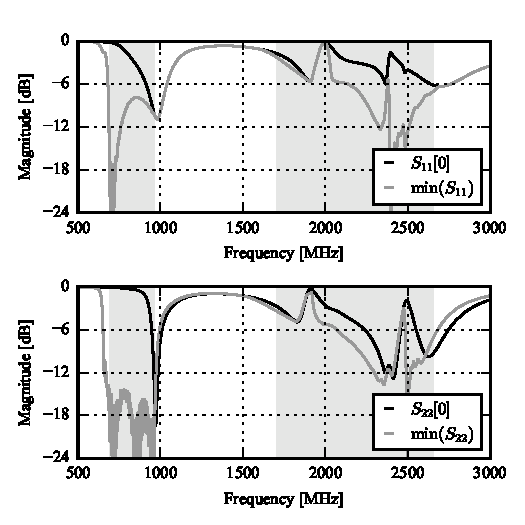
\includegraphics{img/sim/sparams/sparams}
    \caption{Simulated $S$-parameters. Here, $[0]$ marks the minimum capacitance and $\min()$ marks the sweep.}
    \label{fig:sim_sparams}
\end{figure}


%Free space correlation
The correlation simulation is shown in Fig.~\ref{fig:sim_corr}, and is sufficiently low for the high band. However, the antennas are very correlated in the low band. This is decreased when simulated with a user. 
\begin{figure}[tb]
    \centering
    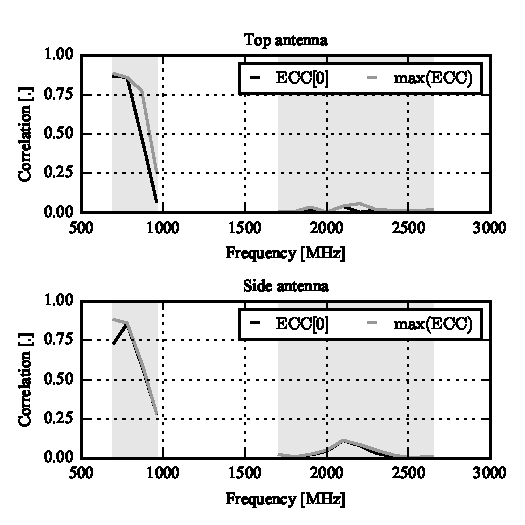
\includegraphics{img/sim/corr/correlation}
    \caption{Simulated envelope correlation coefficient. Here, $[0]$ marks the minimum capacitance and $\max()$ marks the sweep.}
    \label{fig:sim_corr}
\end{figure}


%Free space eff
The efficiency simulation is shown in Fig.~\ref{fig:sim_eff}. For the top antenna, the low band can almost be covered at a \SI{-3}{dB} efficiency. The high band has a notch in \SIrange{1905}{2089}{MHz} but apart from this, the entire high band can be covered at an acceptable efficiency. The side antenna can be tuned to cover the high end of the low band at an efficiency above
\SI{-3}{dB} while the lower part only reaches between \SIrange{-9}{-6}{dB}. The high band has a notch from \SIrange{1825}{2010}{MHz} but has a good efficiency outside this band.
\begin{figure}[tb]
    \centering
    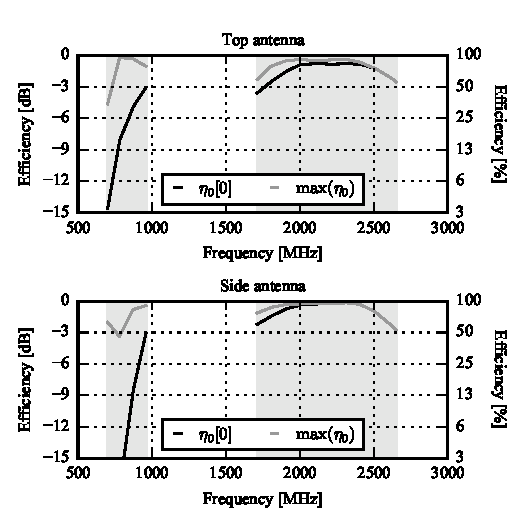
\includegraphics{img/sim/eff/efficiency}
    \caption{Simulated total efficiency. Here, $[0]$ marks the minimum capacitance and $\max()$ marks the sweep. }
    \label{fig:sim_eff}
\end{figure}

%User effects i tabel -> ord 
The user effect simulations showed a general decrease in efficiency and bandwidth and detuned $S$-parameters. The talk-mode simulation shows the worst
detuning and bandwidth coverage compared to the data- and two-hand-mode simulations. The top antenna can still cover the low desired bands at \SI{4}{dB} return loss, while the side antenna is slightly more detuned, covering \SI{630}{MHz} to around \SI{880}{MHz} at \SI{4}{dB} return loss. Generally the correlation is still quite high in the low band with a maximum value of 0.8 in the talk-mode case.

%SAR 
The SAR simulation was performed at 15 discrete frequencies and with a case and a screen. The case is made of plastic with a permittivity of 3, a permeability of 1, and a loss tangent of \num{0.02}. The screen is made of perfect electric conductor (PEC) stitched to the ground plane. The simulations show that both antennas are compliant with the requirement of a maximum SAR of \SI{2}{W/kg}. The top antenna has the highest SAR value of \SI{1.5}{W/kg} in the high band and the side antenna has a maximum SAR value of \SI{0.6}{W/kg} in the high band. 

